%%%%%%%%%%%%%%%%%%%%%%%%%%%%%%%%%%%%%%%%%%%%%%%%%%%%%%%%%%%%%%%%
\begin{frame}[fragile]\frametitle{}
\begin{center}
{\Large Zenoga}


{\tiny (Based on ``Zen Yoga'' by P J Saher And Deep Knowledge YouTube Channel by Dr Ashish Shukla)}
\end{center}
\end{frame}


%%%%%%%%%%%%%%%%%%%%%%%%%%%%%%%%%%%%%%%%%%%%%%%%%%%%%%%%%%%%%%%%
\begin{frame}[fragile]
\frametitle{Prelude}

\begin{columns}[T] % align columns
\begin{column}{.48\textwidth}
\begin{itemize}
\item Mind is divided into 4 sections
	\begin{itemize}
	\item Section 1 : Brain
	\item Section 2 a: RAS
	\item Section 2 b: CCS
	\item Section 3 : Extra Sensory Perceptions
	\item Section 4 : Soul (atman)
	\end{itemize}
\item RAS:
\item CCS: Critical Certain Stage
\item Lower Dimension: 1, 2a
\item Higher Dimension: 2b, 3, 4
\end{itemize}
\end{column}%
\hfill%
\begin{column}{.48\textwidth}
 \begin{center}
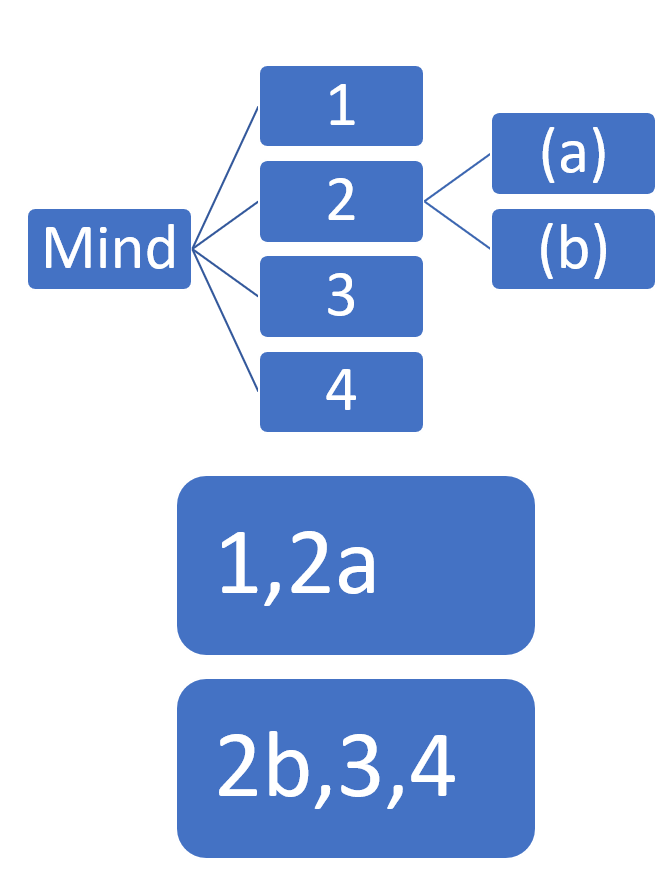
\includegraphics[width=0.9\linewidth,keepaspectratio]{images/zenyoga1}
\end{center}

\end{column}%
\end{columns}
\end{frame}

%%%%%%%%%%%%%%%%%%%%%%%%%%%%%%%%%%%%%%%%%%%%%%%%%%%%%%%%%%%%%%%%
\begin{frame}[fragile]
\frametitle{Section 2a}
\begin{itemize}
\item Intercepts flow from physical body, senses.
\item Adjusts/tones-down/accentuates and sends to thalamus to cortex for decision making.
\item Thus body can report bodily disorders to brain directly without consulting conscious mind.
\item This covers all unconscious/autonomous functions.
\end{itemize}
\end{frame}

%%%%%%%%%%%%%%%%%%%%%%%%%%%%%%%%%%%%%%%%%%%%%%%%%%%%%%%%%%%%%%%%
\begin{frame}[fragile]
\frametitle{Section 2b}
Concentration, Meditation, Intuition.

 \begin{center}
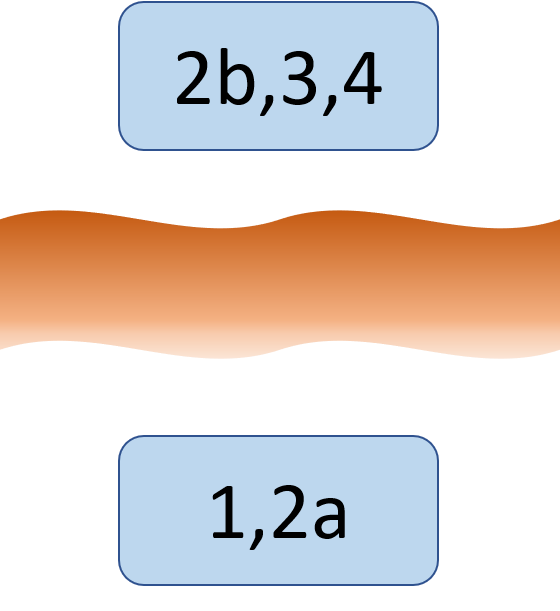
\includegraphics[width=0.35\linewidth,keepaspectratio]{images/zenyoga2}
\end{center}

Goal: Cross the divide (no-mans-land) and go to CCS and further.

\end{frame}

%%%%%%%%%%%%%%%%%%%%%%%%%%%%%%%%%%%%%%%%%%%%%%%%%%%%%%%%%%%%%%%%
\begin{frame}[fragile]
\frametitle{Centers}

\begin{itemize}
\item Section 1:
\begin{itemize}
\item 1. Integrity (I)
\item 2. Emotive (E)
\item 3. Sensual (S)
\item 4. Mobility (M)
\end{itemize}
\item Section 2: 5. Intuition
\item Section 3: 6. Para-mental
\item Section 4: 7. Transcendental
\end{itemize}

\end{frame}


%%%%%%%%%%%%%%%%%%%%%%%%%%%%%%%%%%%%%%%%%%%%%%%%%%%%%%%%%%%%%%%%
\begin{frame}[fragile]
\frametitle{Section 1 Centers}

\begin{itemize}
\item 1. Integrity: through intellectual introspection. ``iih'' - will to know, thinking.
\item 2. Emotive: Evocative of emotions, feelings, ``rajas''.
\item 3. Sensual: Sensuo-vitality, reflexes, drive, longings, ``tamas''.
\item 4. Mobility: muscular, ``manas''.
\end{itemize}


\end{frame}

%%%%%%%%%%%%%%%%%%%%%%%%%%%%%%%%%%%%%%%%%%%%%%%%%%%%%%%%%%%%%%%%
\begin{frame}[fragile]
\frametitle{Noting}

\begin{itemize}
\item Only an enthusiastic life is capable of creativity.
\item Only surface of the ocean are whipped to waves by the winds of ``karma'', its depths are unstirred.
\end{itemize}


\end{frame}

%%%%%%%%%%%%%%%%%%%%%%%%%%%%%%%%%%%%%%%%%%%%%%%%%%%%%%%%%%%%%%%%
\begin{frame}[fragile]
\frametitle{Reality}

\begin{itemize}
\item We believe in what we actually see and hear, but there can be more than that.
\item We can see only between 0.00008 to 0.00009(?) cm. Rest is there but we cant see.
\item Examples: Radio waves which are 20km wavelength, cosmic rays which are $10^{-10}$mm.
\item We can hear only between 30 to 20k per second.
\item Can we still say that we know everything?
\item We are very much Deaf and Blind.
\item By practice of Zenoga, range of perceptions can be increased.
\end{itemize}


\end{frame}

%%%%%%%%%%%%%%%%%%%%%%%%%%%%%%%%%%%%%%%%%%%%%%%%%%%%%%%%%%%%%%%%
\begin{frame}[fragile]
\frametitle{Chapter 1}

\begin{itemize}
\item Drift: Change in thoughts away from the main subject.
\item Types:
\begin{itemize}
\item Un-controllable: Unaware of it, can not recollect
\item Controllable: Can detect and come back to the main subject.
\end{itemize}
\item Mind, if not trained, can not channelize drifts.
\item This drift is not property of the whole mind but one section within it.
\item So, learn to separate sections of mind and understand the functionality.
\end{itemize}


\end{frame}

%%%%%%%%%%%%%%%%%%%%%%%%%%%%%%%%%%%%%%%%%%%%%%%%%%%%%%%%%%%%%%%%
\begin{frame}[fragile]
\frametitle{Chapter 2}
Forms of Consciousness:
\begin{itemize}
\item Simple: like animals, awareness of body. Needed for daily survival.
\item Self: Aware of mental states, sense of self, thoughts.
\item Cosmic: Higher state. Not achieved by logic, reasoning, etc but by stronger awareness.
\item No one has shown practical steps to go from Self to Cosmic consciousness.
\item Even if we get to know the steps, they are difficult to follow. Old patterns are hard to break away from.
\end{itemize}


\end{frame}

%%%%%%%%%%%%%%%%%%%%%%%%%%%%%%%%%%%%%%%%%%%%%%%%%%%%%%%%%%%%%%%%
\begin{frame}[fragile]
\frametitle{Drift Order}
\begin{itemize}
\item Drifts happen in the section of mind that deals with pictures, day-dreams.
\item Typically the come in this order:
\begin{itemize}
\item Sexual
\item Anger
\item Ego
\item Greed
\item Jealousy
\item Arrogance
\item Ignorance
\item Courage
\item Doubt
\item Day dreaming
\end{itemize}
\end{itemize}
\end{frame}

%%%%%%%%%%%%%%%%%%%%%%%%%%%%%%%%%%%%%%%%%%%%%%%%%%%%%%%%%%%%%%%%
\begin{frame}[fragile]
\frametitle{Exercise}
\begin{itemize}
\item Put aside 15-30 minutes in a day to watch the drifts and note them down.
\item Take one thought as the main subject.
\item Let the mind drift.
\item Classify and note the drift.
\item Never try to make your mind ``blank''.
\item Analyze over 3 months, the persistent patterns.
\end{itemize}
\end{frame}

%%%%%%%%%%%%%%%%%%%%%%%%%%%%%%%%%%%%%%%%%%%%%%%%%%%%%%%%%%%%%%%%
\begin{frame}[fragile]
\frametitle{Chapter 3}
\begin{itemize}
\item Brain is a physical entity.
\item Impulses come from various sensory organs, which perturb the nerves/areas in brain. These are called as `thoughts'.
\item Collection of thoughts (or the software/platform, in IMHO) is called as `mind'.
\item Reactions to other minds can be of types:
\begin{itemize}
\item Affinity: love
\item Repulsion: hate
\item Indifference
\end{itemize}
\end{itemize}


\end{frame}

%%%%%%%%%%%%%%%%%%%%%%%%%%%%%%%%%%%%%%%%%%%%%%%%%%%%%%%%%%%%%%%%
\begin{frame}[fragile]
\frametitle{Mind as a Cloth}
\begin{itemize}
\item Thoughts are strands
\item Emotions are the colors
\item Repetition or habit strengthens and makes cloth durable.
\item Quality of thoughts correspond to smoothness or roughness of the cloth.
\item Grey matter, attitude, thought process: Shape of the cloth
\item Likes/Dislikes: fashion of the cloth.
\end{itemize}

Constant daily practice can change the properties of the cloth.
\end{frame}

%%%%%%%%%%%%%%%%%%%%%%%%%%%%%%%%%%%%%%%%%%%%%%%%%%%%%%%%%%%%%%%%
\begin{frame}[fragile]
\frametitle{Chapter 4}
\begin{itemize}
\item Incoming impulses are decoded in brain as Pure Mind Energy, which are divided into:

\begin{itemize}
\item Held: thoughts suppressed
\item Words: expressed as words or mental pictures, day dreaming.
\item Actions: Something is done by them, movements.
\end{itemize}
\item As per Patanjali, there are 5 states (`vrutti') of mind (`chitta'):
\begin{itemize}
\item Correct Knowledge
\item Incorrect Knowledge
\item Fancy
\item Passivity (sleep)
\item Memory
\end{itemize}
\item Mind can be controlled (``chitta vrutti nirodh:'') by efforts, detachment.
\item Peace of mind can be brought by regulation of ``prana'' (breath).
\end{itemize}

\end{frame}

%%%%%%%%%%%%%%%%%%%%%%%%%%%%%%%%%%%%%%%%%%%%%%%%%%%%%%%%%%%%%%%%
\begin{frame}[fragile]
\frametitle{Chapter 5: Sleep}
\begin{itemize}
\item Types of Sleep are:
\resizebox{\textwidth}{!}{%
  \begin{tabular}{|c|c|c|c|c|}
  \hline
  Type & Beneficial? &Timing&Vibrational Color built in Body\\
  \hline
  Very Intense 	& 	Very beneficial	&	Midnight to 4am	&	Pale Blue\\
  Intense     	&	Beneficial		& 	11pm to Midnight, 4 to 5am	&	Pink\\
  Indifferent  	&	Does not add to energy	& 9 to 11pm, 5 to 7am &Green\\
  Wasting		& 	Losing energy & 7am to 12 noon & Yellow (dark) \\
  Damaging		& 	Bad to nerves &  12 noon to 4 pm & Orange (deep)\\
  Highly Damaging & Sickness, disease & 4pm to 9pm&  Red (deep)\\
  
  
  \hline
  \end{tabular}
} % end of scope of "\resizebox"  directive

\item Resting and sleeping are two different things.
\item 11pm to 5pm should be considered as a good time for sleep.
\end{itemize}
\end{frame}








%%%%%%%%%%%%%%%%%%%%%%%%%%%%%%%%%%%%%%%%%%%%%%%%%%%%%%%%%%%%%%%%
\begin{frame}[fragile]\frametitle{}
\begin{center}
{\Large Notes from Other References}
\end{center}
\end{frame}


%%%%%%%%%%%%%%%%%%%%%%%%%%%%%%%%%%%%%%%%%%%%%%%%%%%%%%%%%%%%%%%%
\begin{frame}[fragile]
\frametitle{``Introduction To Three Step Rhythmic Breathing(3SRB)'' by Mr.Deepak Dhingra}


\begin{itemize}
\item Yaksh : ``What's the most delusion that humans have?''
\item Yudhishthiara: ``People live life as if they are not going to die''.
\item Its inevitable. No one has control. 
\item Only sometimes externally.
\item But we have no control internally. 
\end{itemize}
\end{frame}


%%%%%%%%%%%%%%%%%%%%%%%%%%%%%%%%%%%%%%%%%%%%%%%%%%%%%%%%%%%%%%%%
\begin{frame}[fragile]
\frametitle{Mind}
\begin{itemize}
\item None of the internal organs behave the way we want. 
\item Including brain!! although we believe we have control on that
\item Brain is just another organ, a hardware. And mind is the energy/software that runs on it.
\item Proof: After death, hardware remains, but the software/energy is shutdown, so cant function.
\end{itemize}
\end{frame}



%%%%%%%%%%%%%%%%%%%%%%%%%%%%%%%%%%%%%%%%%%%%%%%%%%%%%%%%%%%%%%%%
\begin{frame}[fragile]
\frametitle{Free Will?}

\begin{itemize}
\item We have no control internally. Many centers are producing impulses. Most of the organ functioning is autonomous
\item Thus we cannot control mind, but we have to bring them to rhythm, balance.
\item As per Pantanjali, daily, out of 13k impulses 120 go to brain. Rest are used to keep system working. Out of 120 to brain, 12 are per second, Only one becomes a thought. This just one more theory. May ignore. Just a model.
% \item We are interpreting life our way and not how it is
\end{itemize}
\end{frame}

%%%%%%%%%%%%%%%%%%%%%%%%%%%%%%%%%%%%%%%%%%%%%%%%%%%%%%%%%%%%%%%%
\begin{frame}[fragile]
\frametitle{Mind}
\begin{itemize}
\item As per Patanjali, Breathing is one way to control the mind.
\item Breathing happens as per emotions, eg. anger.
\item Can controlling breathing control emotions? Patanjali says, Yes.
\item Mind (Software) is run by breath. When Breath stops, its called death.
\item Need Deep, Rhythmic and Belly breathing
\end{itemize}
\end{frame}

%%%%%%%%%%%%%%%%%%%%%%%%%%%%%%%%%%%%%%%%%%%%%%%%%%%%%%%%%%%%%%%%
\begin{frame}[fragile]
\frametitle{3SRB (3 Step Rhythmic Breathing )}

Technique

\begin{itemize}
\item Both chest and abdomen are raised and lowered together equally.
\item Note: You can lie down in front of the mirror with two heavy books one on the chest and the other on the abdomen. 
\item Check whether both move together.
\end{itemize}

\tiny{(Ref: https://www.3srb.org/3srb/how-to-practise-3srb.html )}
\end{frame}

%%%%%%%%%%%%%%%%%%%%%%%%%%%%%%%%%%%%%%%%%%%%%%%%%%%%%%%%%%%%%%%%
\begin{frame}[fragile]
\frametitle{3SRB (3 Step Rhythmic Breathing )}

Volume

\begin{itemize}
\item The breath is full from neck to naval, i.e. the upper, middle and lower abdomen are filled to normal capacity
\item The quantum of air inhaled and exhaled is what is usually normal to us neither too much nor too forceful, since normal 3SRB is not an exercise but a process of correct breathing. 
\item Note: Initially, to establish the rhythm your breath will be deeper. Once, the technique and volume is mastered, then the volume of the breath will be normal as you breath today.
\end{itemize}
\end{frame}


%%%%%%%%%%%%%%%%%%%%%%%%%%%%%%%%%%%%%%%%%%%%%%%%%%%%%%%%%%%%%%%%
\begin{frame}[fragile]
\frametitle{3SRB (3 Step Rhythmic Breathing )}

Rhythm

\begin{itemize}
\item In 3 sec out 2 sec | one hand chest one hand on belly| equal volume. No jerks. 
\item  While counting its 1-2-3 (4) 5-6. Here, at ``4'' it is the turn of breath. Is not counted but just understood. Later, same but with deep breathing, and fast
\item 12 cycles a minute to start with then to 24 and 36.
\item  Increase the duration of practice by 5 minutes every fortnight until 6 months time and until one hour of conscious 3SRB is reached.
\end{itemize}
\end{frame}


%%%%%%%%%%%%%%%%%%%%%%%%%%%%%%%%%%%%%%%%%%%%%%%%%%%%%%%%%%%%%%%%
\begin{frame}[fragile]
\frametitle{3SRB by ShriRajen Vakil}


\begin{itemize}
\item Deep Chest breathing: Both hands on chest. Let breath come in and push chest out. 36 times a minute. Only for a minute. On rhythm 123-56. Area of anger, jealousy stored so far.
\item Deep Stomach breathing: Both hands on belly. Let breath come in and push belly out. On exhale push belly in. 36 times a minute. Only for a minute. On rhythm 123-56. Area of fear and worry for future.
\item Paschimottanasan breathing: Head up. Both chest and stomach should come out on breath in. 36 times a minute. Only for a minute. On rhythm 123-56. For backbone, the channel for energy to go up.
\item Take breath in 5 installments and breath in through mouth forcefully. 12345-Out
\item Breath in 5 seconds, hold 5, empty 5, hold 5. 3 such rounds.
\item Inhale, hold breath, touch chin, swallow 5 times. Area of Pain.

\end{itemize}
\end{frame}

%%%%%%%%%%%%%%%%%%%%%%%%%%%%%%%%%%%%%%%%%%%%%%%%%%%%%%%%%%%%%%%%
\begin{frame}[fragile]\frametitle{}
\begin{center}
{\Large Conclusion}
\end{center}
\end{frame}



%%%%%%%%%%%%%%%%%%%%%%%%%%%%%%%%%%%%%%%%%%%%%%%%%%%%%%%%%%%%%%%%
\begin{frame}[fragile]
\frametitle{Summary To-Dos}
\begin{itemize}
\item Breath: Three Step Rhythmic Breathing
\item Food: lessen intake slowly to 1 time, be aware, get rid off addiction
\item Drift: Watch thoughts-wavering, Put in Fear/Anger/Sex/Hope/Jealousy
\item Walking with Awareness: 
\item Corrective methods: replace negative with positive thoughts
\item Sleep: 11 pm to 5 am. Other times do 3 step breathing
\item Reading
\item Sex Moderation
\item Awareness of Eyes: watch carefully, focus
\item Awareness of Ears: listen carefully, don't drift
\end{itemize}
\end{frame}